% !TEX TS-program = pdflatex
% !TEX encoding = UTF-8 Unicode

% This is a simple template for a LaTeX document using the "article" class.
% See "book", "report", "letter" for other types of document.

\documentclass[11pt]{article} % use larger type; default would be 10pt

\usepackage[utf8]{inputenc} % set input encoding (not needed with XeLaTeX)

%%% Examples of Article customizations
% These packages are optional, depending whether you want the features they provide.
% See the LaTeX Companion or other references for full information.

%%% PAGE DIMENSIONS
\usepackage{geometry} % to change the page dimensions
\geometry{letterpaper} % or letterpaper (US) or a5paper or....
% \geometry{margin=2in} % for example, change the margins to 2 inches all round
% \geometry{landscape} % set up the page for landscape
%   read geometry.pdf for detailed page layout information

\usepackage{graphicx} % support the \includegraphics command and options

% \usepackage[parfill]{parskip} % Activate to begin paragraphs with an empty line rather than an indent

%%% PACKAGES
\usepackage{booktabs} % for much better looking tables
\usepackage{array} % for better arrays (eg matrices) in maths
\usepackage{paralist} % very flexible & customisable lists (eg. enumerate/itemize, etc.)
\usepackage{verbatim} % adds environment for commenting out blocks of text & for better verbatim
\usepackage{subfig} % make it possible to include more than one captioned figure/table in a single float
% These packages are all incorporated in the memoir class to one degree or another...

%%% HEADERS & FOOTERS
\usepackage{fancyhdr} % This should be set AFTER setting up the page geometry
\pagestyle{fancy} % options: empty , plain , fancy
\renewcommand{\headrulewidth}{0pt} % customise the layout...
\lhead{}\chead{}\rhead{}
\lfoot{}\cfoot{\thepage}\rfoot{}

%%% SECTION TITLE APPEARANCE
\usepackage{sectsty}
\allsectionsfont{\sffamily\mdseries\upshape} % (See the fntguide.pdf for font help)
% (This matches ConTeXt defaults)

%%% ToC (table of contents) APPEARANCE
\usepackage[nottoc,notlof,notlot]{tocbibind} % Put the bibliography in the ToC
\usepackage[titles,subfigure]{tocloft} % Alter the style of the Table of Contents
\renewcommand{\cftsecfont}{\rmfamily\mdseries\upshape}
\renewcommand{\cftsecpagefont}{\rmfamily\mdseries\upshape} % No bold!

%%% END Article customizations

%%% The "real" document content comes below...

\title{Portable Tilt Meter Unit Instruction Guide}
\author{J.R. Leeman}
\date{} % Activate to display a given date or no date (if empty),
         % otherwise the current date is printed 

\begin{document}
\maketitle

\section{Kit Components}

This kit contains all components needed to record two axis tilt meter data in the field, provided an external 7-23 VDC power source. Before shipping this kit, be sure that all kit components are in place.

\begin{enumerate}
\item Unit power cord x 1
\item GPS Antenna x 1
\item Tilt meter logger x 1
\item Tilt meter sensor x 1
\item Tilt meter computer connection cable x1
\item Micro SD Card and Adapter x 1
\item Sealing putty x 1
\item Instruction Manual x 1
\end{enumerate}

% Figure %
\begin{figure}
	\centering
		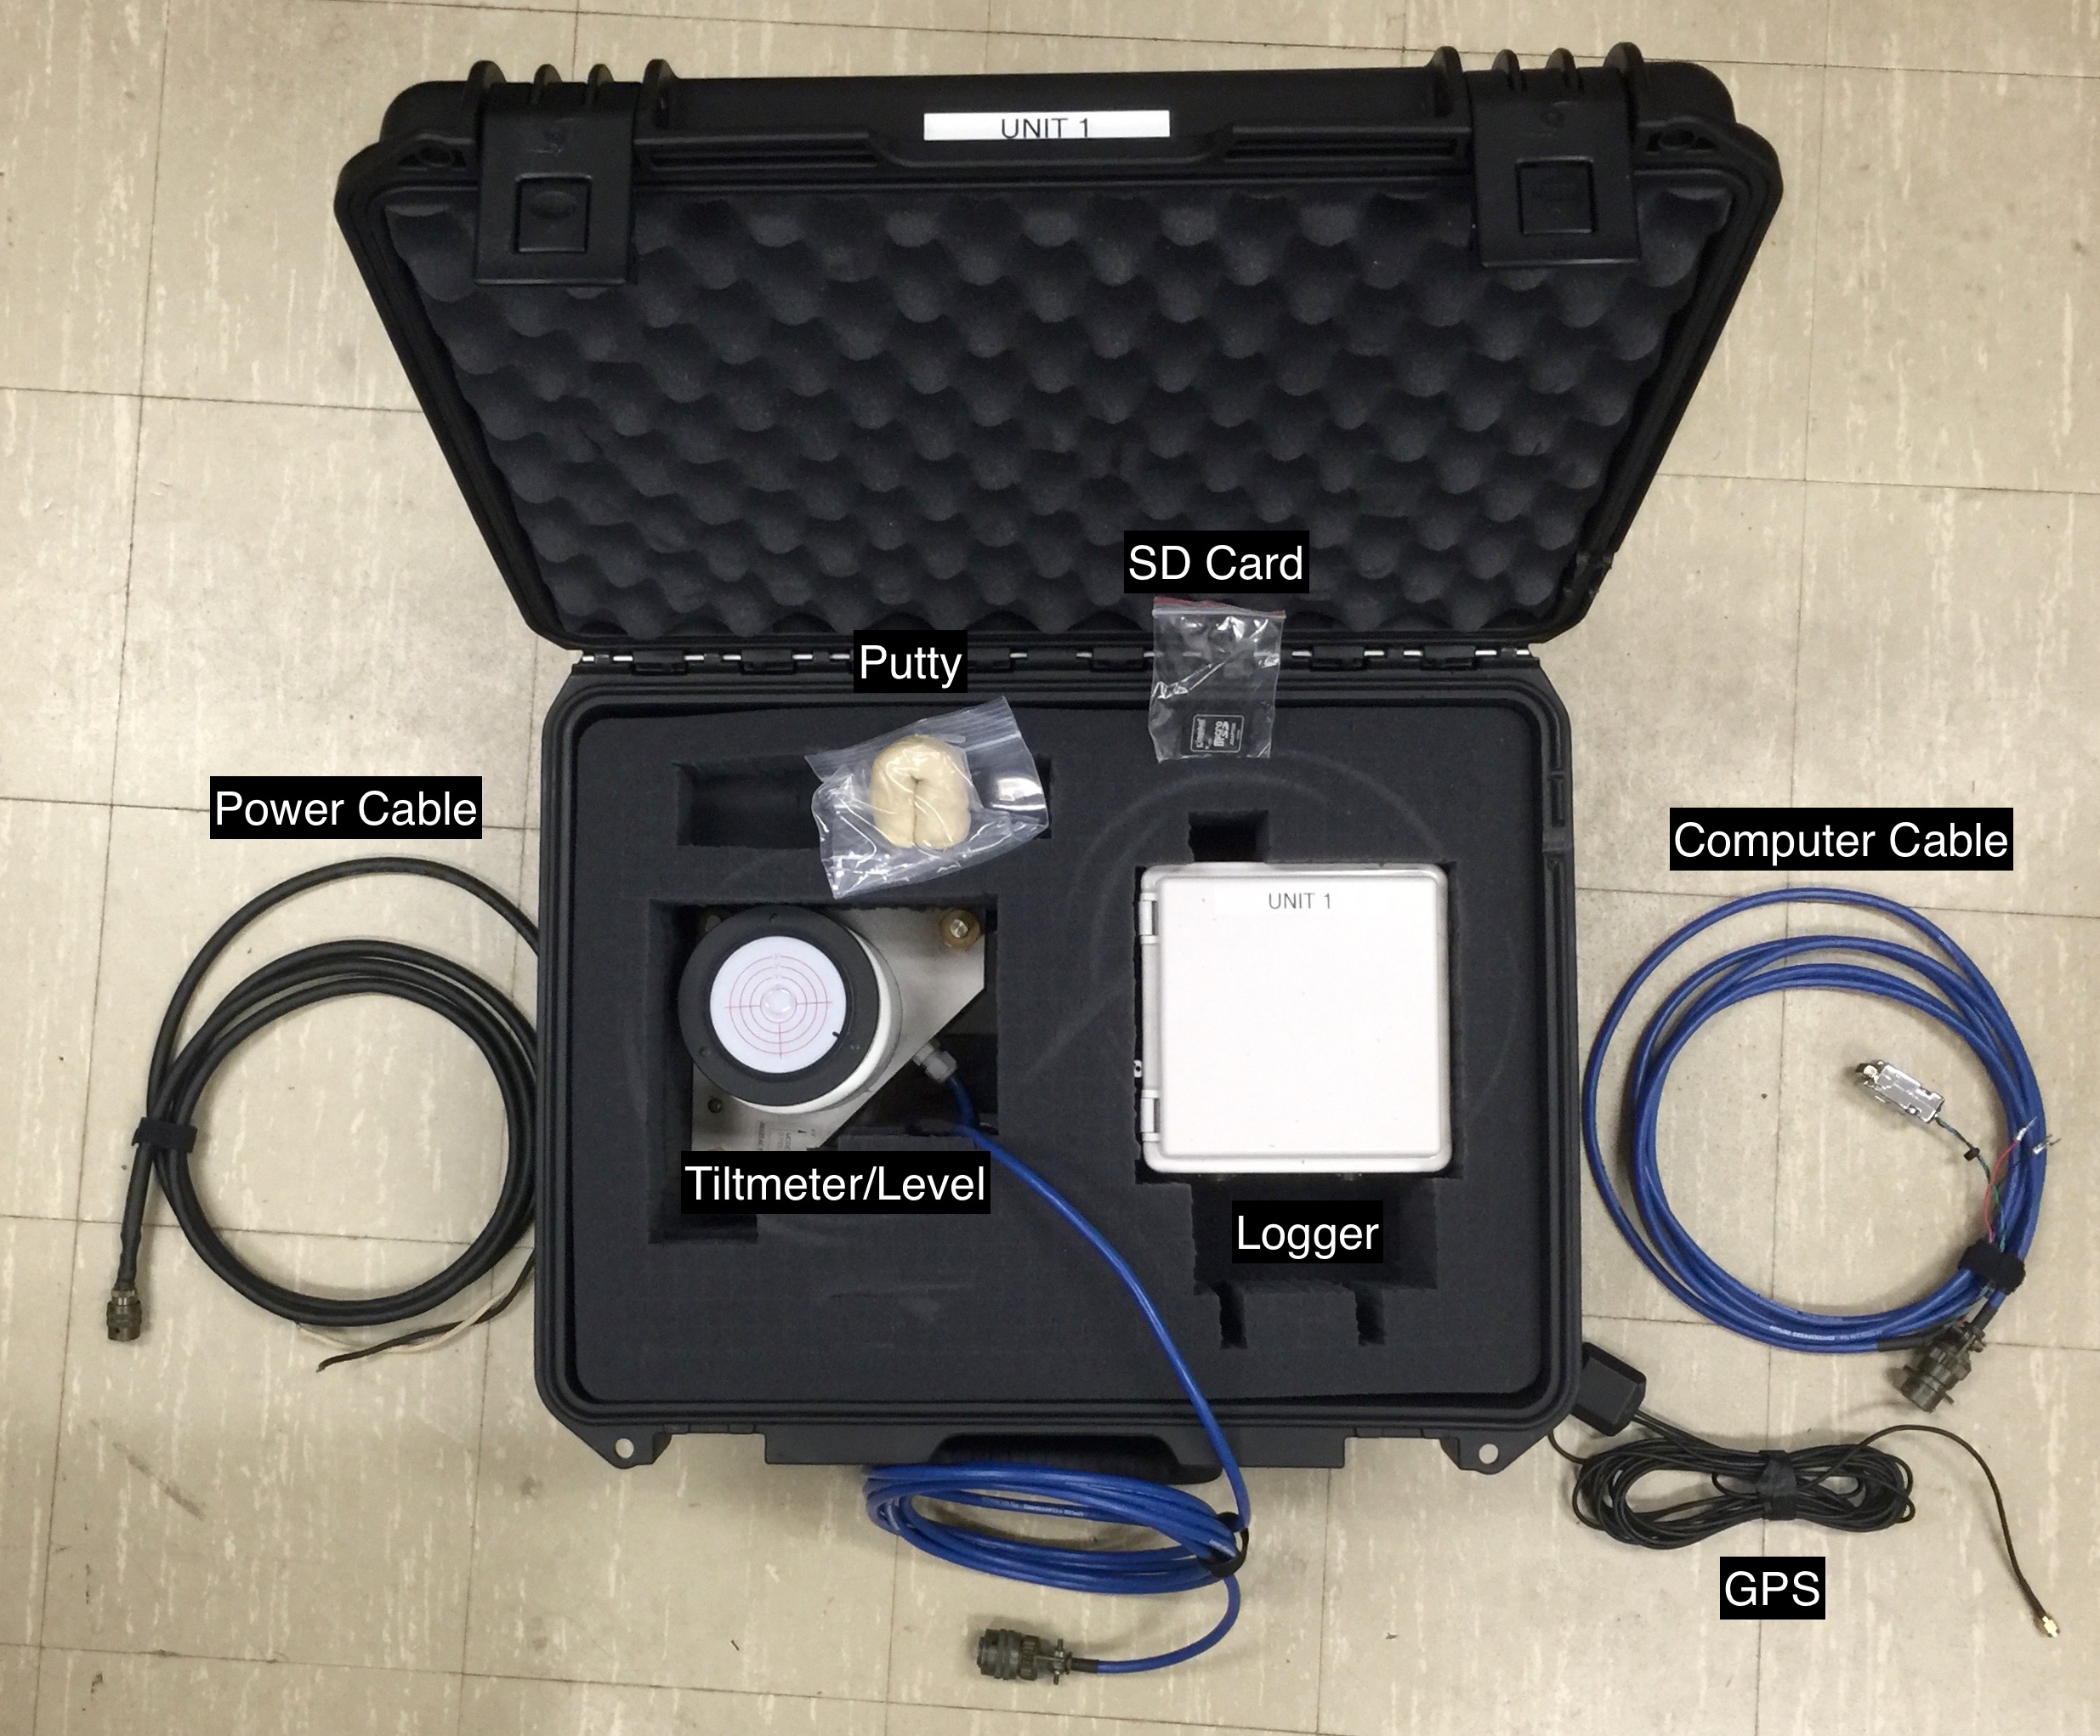
\includegraphics[scale=0.1]{kit_annotated.jpg}
   	\caption{Kit contents essential for a deployment.}
  	\label{kit}
\end{figure}
% End Figure %

\newpage
\section{Setup}
Carefully follow these instructions to ensure a reliable and useful field deployment of the portable tilt meter package. 

\begin{enumerate}
\item Select a location on stable, flat ground.
\item Place the equipment case and remove the cables and GPS antenna.
\item Level the tilt meter with the bubble level. Loosen the brass lock nuts if needed. Tighten lock nuts finger tight when level. Recheck level!
\item \emph{Optional:} Connect the computer link cable to power and the serial port of a computer. Connect the cable to the tilt meter.
\item \emph{Optional:} Open a serial terminal utility and connect to the tilt meter (9800,N,0,1).
\item \emph{Optional:} Enter *9900XY into the terminal and press return (if no response make sure your terminal is sending $<$CR$><$LF$>$ at the end of the serial sequence).
\item \emph{Optional:} The tilt meter should return the x tilt, y tilt, temperature, and its serial number.
\item \emph{Optional:} Adjust the level of the until and repeat the process above until the unit is nearly centered in the measurement range. Use the lock nuts to secure the setting.
\item \emph{Optional:} Remove power and disconnect the computer cable. 
\item Connect the tilt meter cable to the tilt port on the logger.
\item Open the logging unit with the two latches.
\item Ensure that the GPS and tilt serial switches and in the positions shown in figure \ref{labeled_box}.
\item Connect the GPS antenna to the antenna connector on the logger and place it outside the box.
\item Insert a formatted (FAT32) SD card into the top SD card holder.
\item Check that a backup battery is inserted into the coin cell battery holder. This battery lasts for years and is a CR1220. 
\item Connect the power cable to a 7-23 VDC power source (battery, etc). Black to ground and white to positive. DO NOT REVERSE THESE!
\item Connect the power cable to the logging box. 
\item Large red and green LEDs will illuminate to indicate the the logger is completing setup routines. These lights flash twice to verify that setup was completed successfully (about 20-30 seconds). This process may repeat if the GPS lock takes longer than 30 seconds. 
\item The small yellow LED labeled L13 should flash once per second. The green PWR LED should be on solid. The red FIX led should flash approximately once every 15 seconds once GPS lock is established. If any other lights are on or flashing the unit is not functioning correctly. Check the error codes.
\item Close and seal the logging electronics (white) box.
\item Carefully route the power and GPS antenna cables though the slots in the case. Seal with a small strip of putty if necessary.
\item Stow all extra cables.
\item Close the case gently so the unit stays level and lock the case shut. Deployment is complete.
\end{enumerate}

% Figure %
\begin{figure}
	\centering
		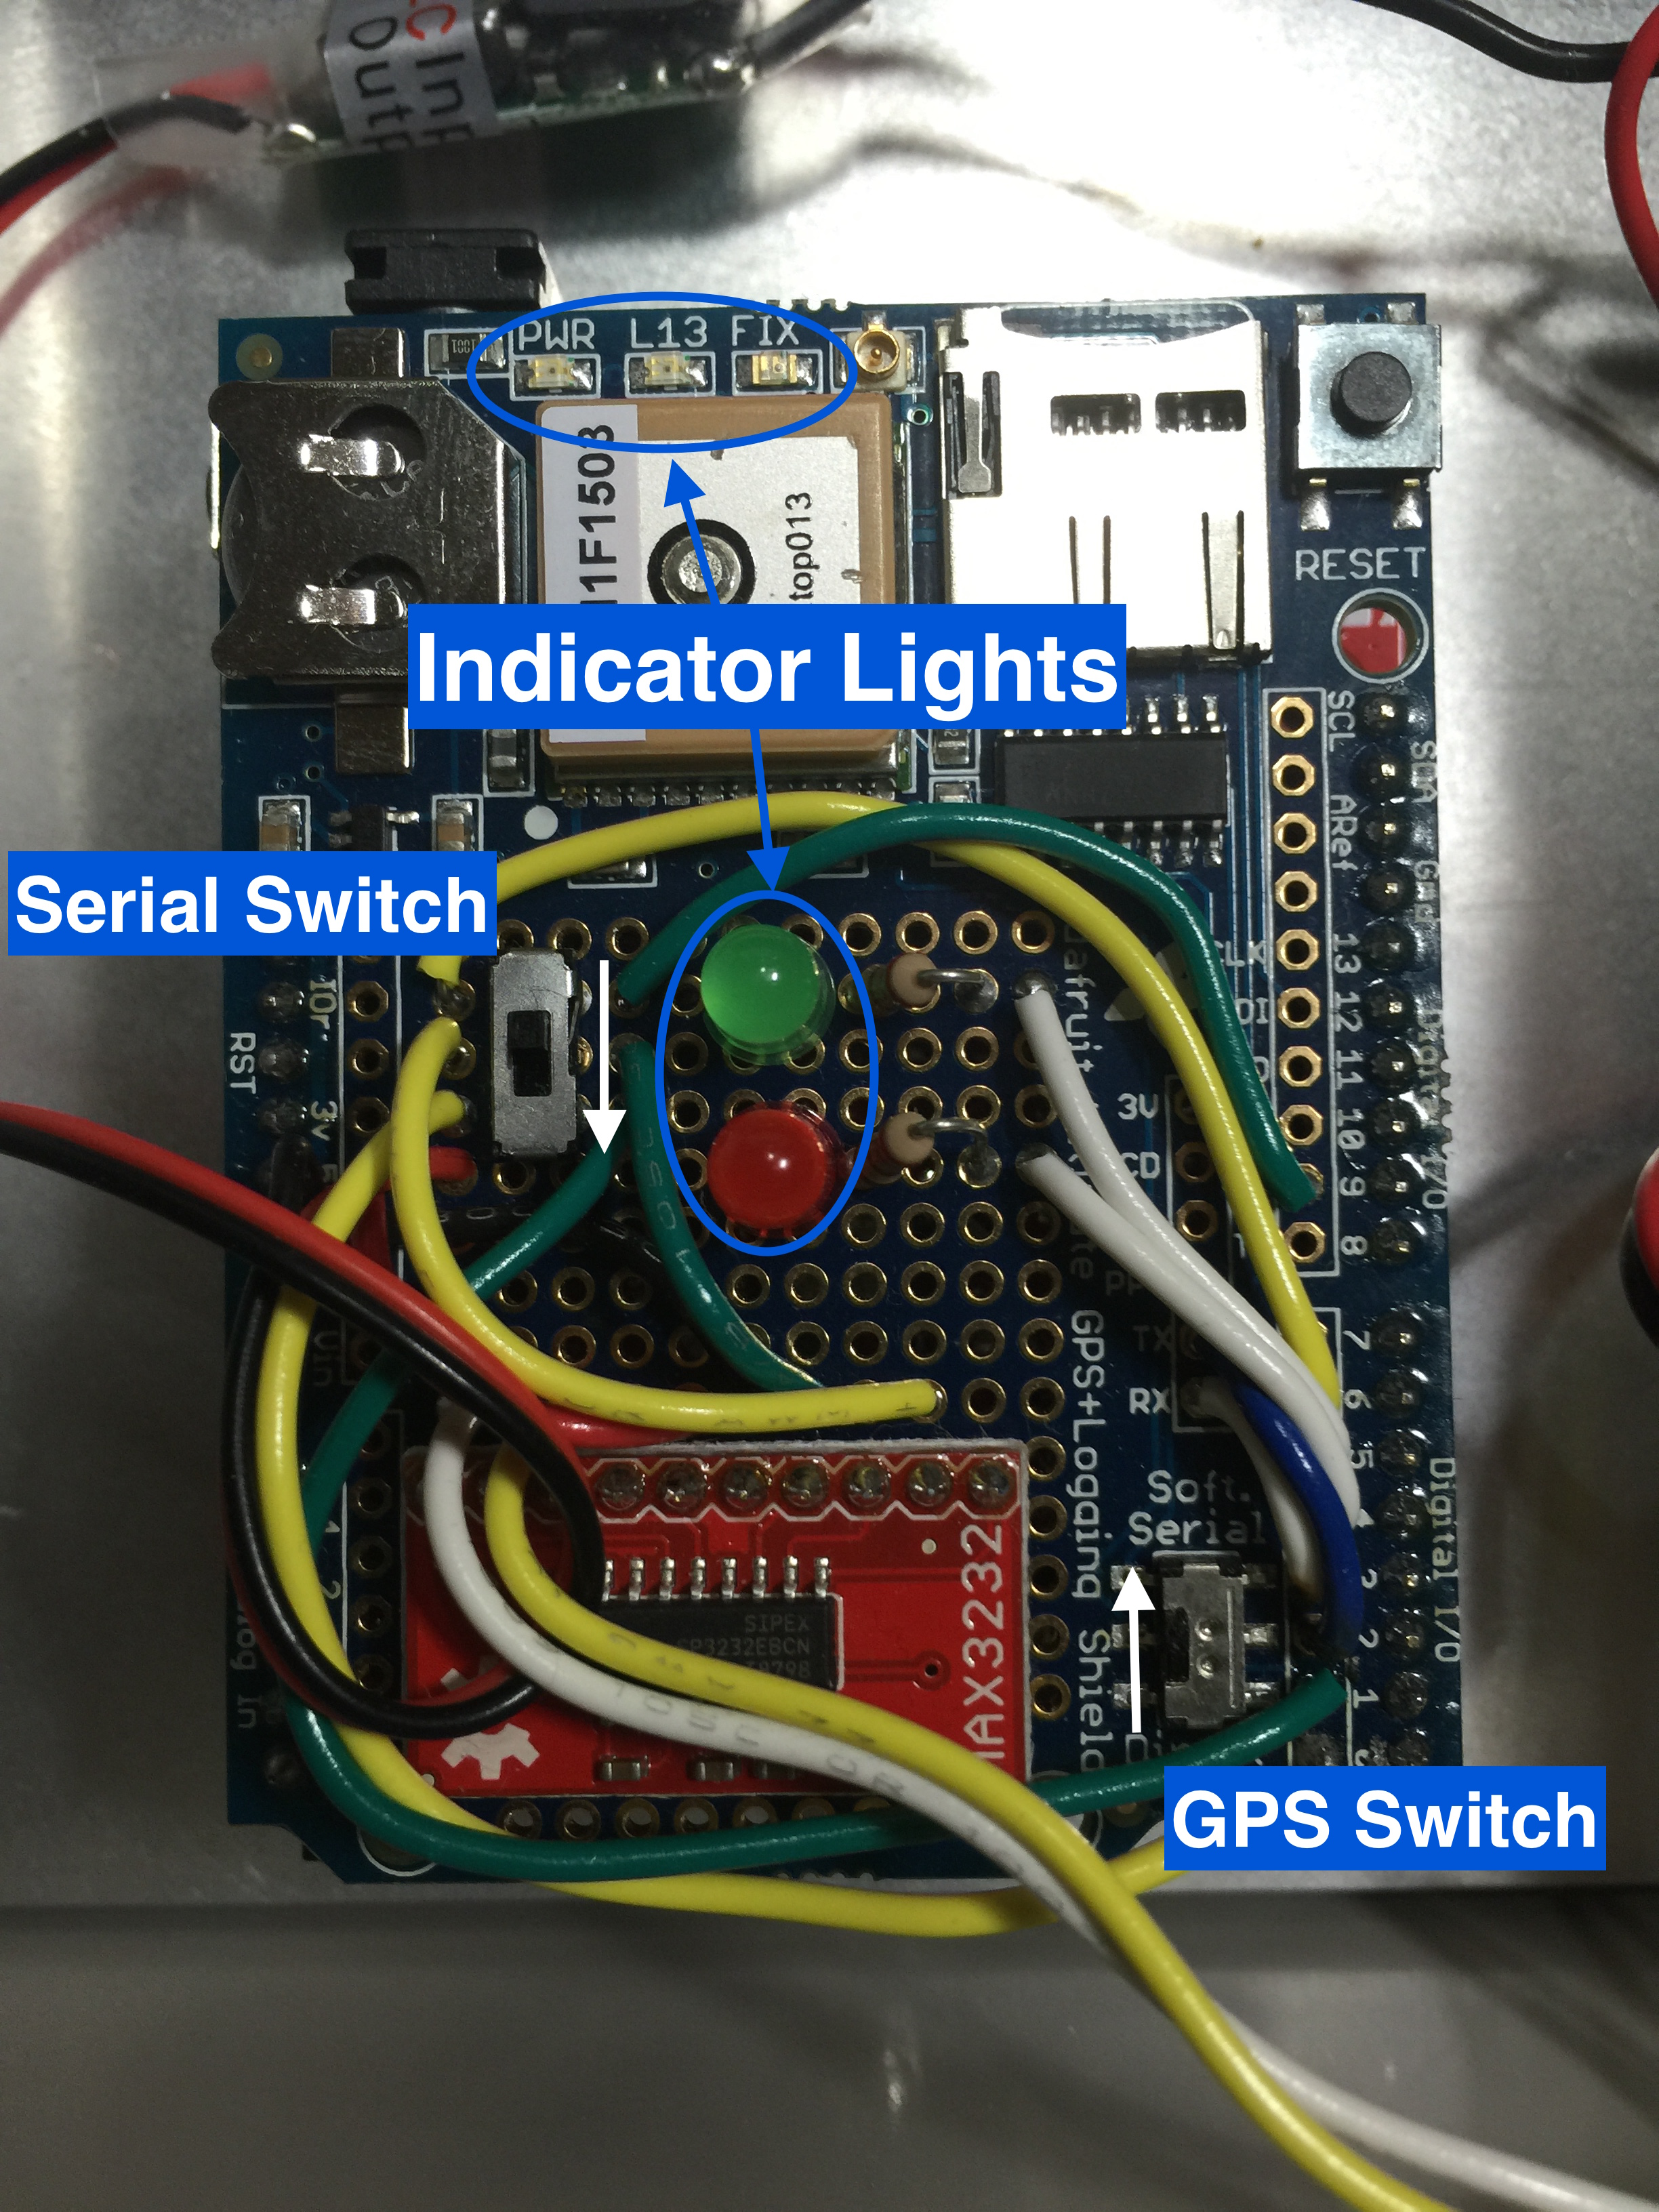
\includegraphics[scale=0.1]{board.jpg}
   	\caption{Essential controls and indicators in the logger box.}
  	\label{labeled_box}
\end{figure}
% End Figure %

\newpage
\section{Take Down}
Take down procedures render the unit safe and prepare it for shipping. Failure to follow these instructions could result in damage or data loss.

\begin{enumerate}
\item Carefully open the case.
\item Remove power from the logging unit by disconnecting the power cable.
\item Disconnect the power cable from the power source.
\item Disconnect the tilt meter cable from the logging unit.
\item Disconnect the GPS antenna from the logging unit. Stow.
\item Open the logging unit and recover the SD card with your data on it.
\item Seal and replace the logging unit.
\item Carefully wind, bind, and replace all cables and materials.
\item Seal the box. Take down is complete.
\end{enumerate}

\newpage
\section{Error Codes}

\begin{center}
    \begin{tabular}{ |c|c|}
    \hline
    Error Code & Error Description\\
    \hline
    1 red flash &  Cannot open file to write on SD card.\\
    \hline
    2 red flashes &  Cannot start SD card, check card and formatting.\\
    \hline
    3 red flashes &  Error writing GPS data to SD card.\\
    \hline
    4 red flashes &  Error writing tilt data to SD card.\\
    \hline
    red and green simultaneous flashes &  Check serial switch positions.\\
    \hline
    \end{tabular}
\end{center}

\section{Troubleshooting}
When encountering problems with the unit, the following steps will solve most issues.

\begin{itemize}
\item Check all connectors for cleanliness and firm connection. Clean if necessary.
\item Verify that tilt meter can be read from computer interface.
\item Check that SD card is inserted into the right slot and is FAT32 formatted.
\item Verify the position of the two serial switches on the logging unit.
\item Power cycle the unit.
\end{itemize}

\end{document}
